% o \label{codigo} serve para podermos fazer referencias para algo numerado, 
% como capitulos, tabelas, figuras, etc. 
% Quando colocamos o comando \ref{codigo}. o compilador troca o \ref{codigo}
% pelo numero atribuido ao \label{}
% ex. \label{tabelaLegal}
%   A tabela \ref{tabelaLegal} mostra que...
% vai ser substituido por
%   A tabela 2 mostra que

\chapter{Desenvolvimento}\label{cap-desenvolvimento}

Segundo o processo iterativo de desenvolvimento descrito na metodologia, este projeto evoluiu ao longo de várias etapas de crescente complexidade.


% ---
\section{Objetivo e formulação do problema}\label{sec-objetivos-formulacao-problema}
% ---

Foi inicialmente elaborada uma enunciação geral do problema a ser resolvido: a criação de um jogo digital que, valendo-se de técnicas de realidade virtual, oferecesse uma experiência imersiva e educativa a crianças de 8 a 12 anos de idade, de acordo com o recorte selecionado descrito da seção \ref{cap-teoria} de **Teoria**. Tendo essa enunciação como base, pôde-se decidir a respeito de restrições, e do escopo que guiariam as etapas seguintes de conceituação do projeto.

% ---
\subsection{Delimitação do escopo}\label{subsec-delimitacao-escopo}
% ---
TODO

% ---
\subsection{Recorte do público alvo}\label{subsec-recorte-publico-alvo}
% ---

Em primeiro lugar, optou-se por restringir os equipamentos e tecnologias a serem empregados, de modo a facilitar a acessibilidade e adoção em sala de aula e diminuir os custos implantação, sem que a experiência desejada tivesse de ser sacrificada. Isso levou à escolha do uso do Google Cardboard como dispositivo principal de realidade virtual, por seu baixo custo comparado a demais alternativas de mercado, e sua integração a dispositivos móveis que, em muitos casos, já estariam ao alcance dos alunos, ou poderiam ser providenciados sem um grande impacto orçamentário.

Em adição ao Cardboard, optou-se pela implemntação do dispositivo detector de gestos manuais Leap Motion como forma de *input* principal para o jogo, com a vantagem de ser uma alternativa de custo aceitável, capaz de providenciar uma experiência bastante direta na interação do aluno com o mundo do jogo, uma vez que permite que movimentos do jogador no mundo real sejam traduzidos em ações do mundo virtual, permitindo abstrair oos dispositivos de entrada e saída por completo, e mantendo a imersão e engajamento.

Por fim, como restrição adicional, a ferramenta Unity foi escolhida como *engine* de desenvolvimento do jogo, por sua fácil integração ao hardware escolhido, e seu paradigma de desenvolvimento em mais alto nível do que as demais alternativas disponíveis, o que permitiria ao grupo focar-se na conceituação e implementação do jogo em si, sem prender-se a eventuais problemas relativos à configuração e uso do hardware, criação de APIs próprias ou preocupações com elementos mais elementares da criação de um jogo digital.

% ---
\section{Brainstorming e seleção do conceito do jogo}\label{sec-brainstorming-conceito}
% ---

Com a enunciação do problema e as restrições de implementação bem definidas e acordadas pelo grupo, pôde-se passar para a etapa seguinte do desenvolvimento, o *brainstorm*, durante o qual várias ideias foram debatidas e exploradas pelos membros do grupo. Nesta fase, diversas propostas foram feitas para uma solução que fizesse um bom uso dos recursos de realidade virtuais disponíveis e gerasse um projeto adequado ao público alvo selecionado, resultando em um jogo intuitivo, divertido que capaz de transmitir os conceitos de lógicos e cognitivos relevantes.

As ideias geradas variaram desde jogos de um ritmo mais acelerado, no qual um jogador teria que categorizar elementos abstratos o mais rápido que pudesse - segundo características como cor, formato e tamanho - até experiências nas quais pressões de tempo e condições de falha estavam copletamente ausentes, como jogos de resolução de quebra-cabeças tridimensionais.

\begin{figure}[h]
	\centering
	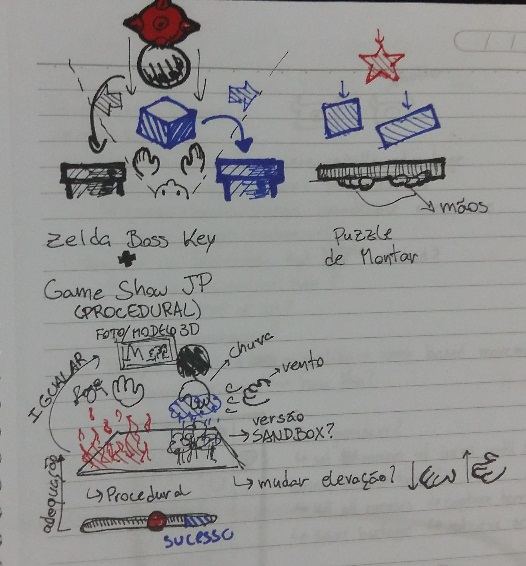
\includegraphics[width=0.5\textwidth]{first_concepts}
	\caption{primeiro rascunho do jogo}
\end{figure}

Por fim, uma análise cuidadosa das limitações das tecnologias escolhidas, aliada a uma preocupação em manter o jogo intuitivo e imersivo levaram o grupo a um design mais diretamente análogo ao mundo real, gerando um jogo no qual o jogador manipularia características de uma pequena configuração geológica tridimensional, de forma a manipulá-la para chegar a um determinado estado pré-definido.

Neste jogo, as crianças se deparariam com um terreno digital composto por acidentes geográficos como planaltos, depressões, corpos d'água e formações magmáticas, e poderiam modificá-lo a partir de gestos manuais simples que controlassem a elevação, precipitação, movimentação do ar, entre outros. Este terreno seria subdivido em unidades cúbicas que poderiam ser manipuladas individualmente, fornecendo uma resolução suficiente para que configurações diversas e interessantes pudessem ser construídas, mas sem exigir uma precisão incompatível com os dispositivos de entrada e saída escolhidos.

\begin{figure}[h]
	\centering
	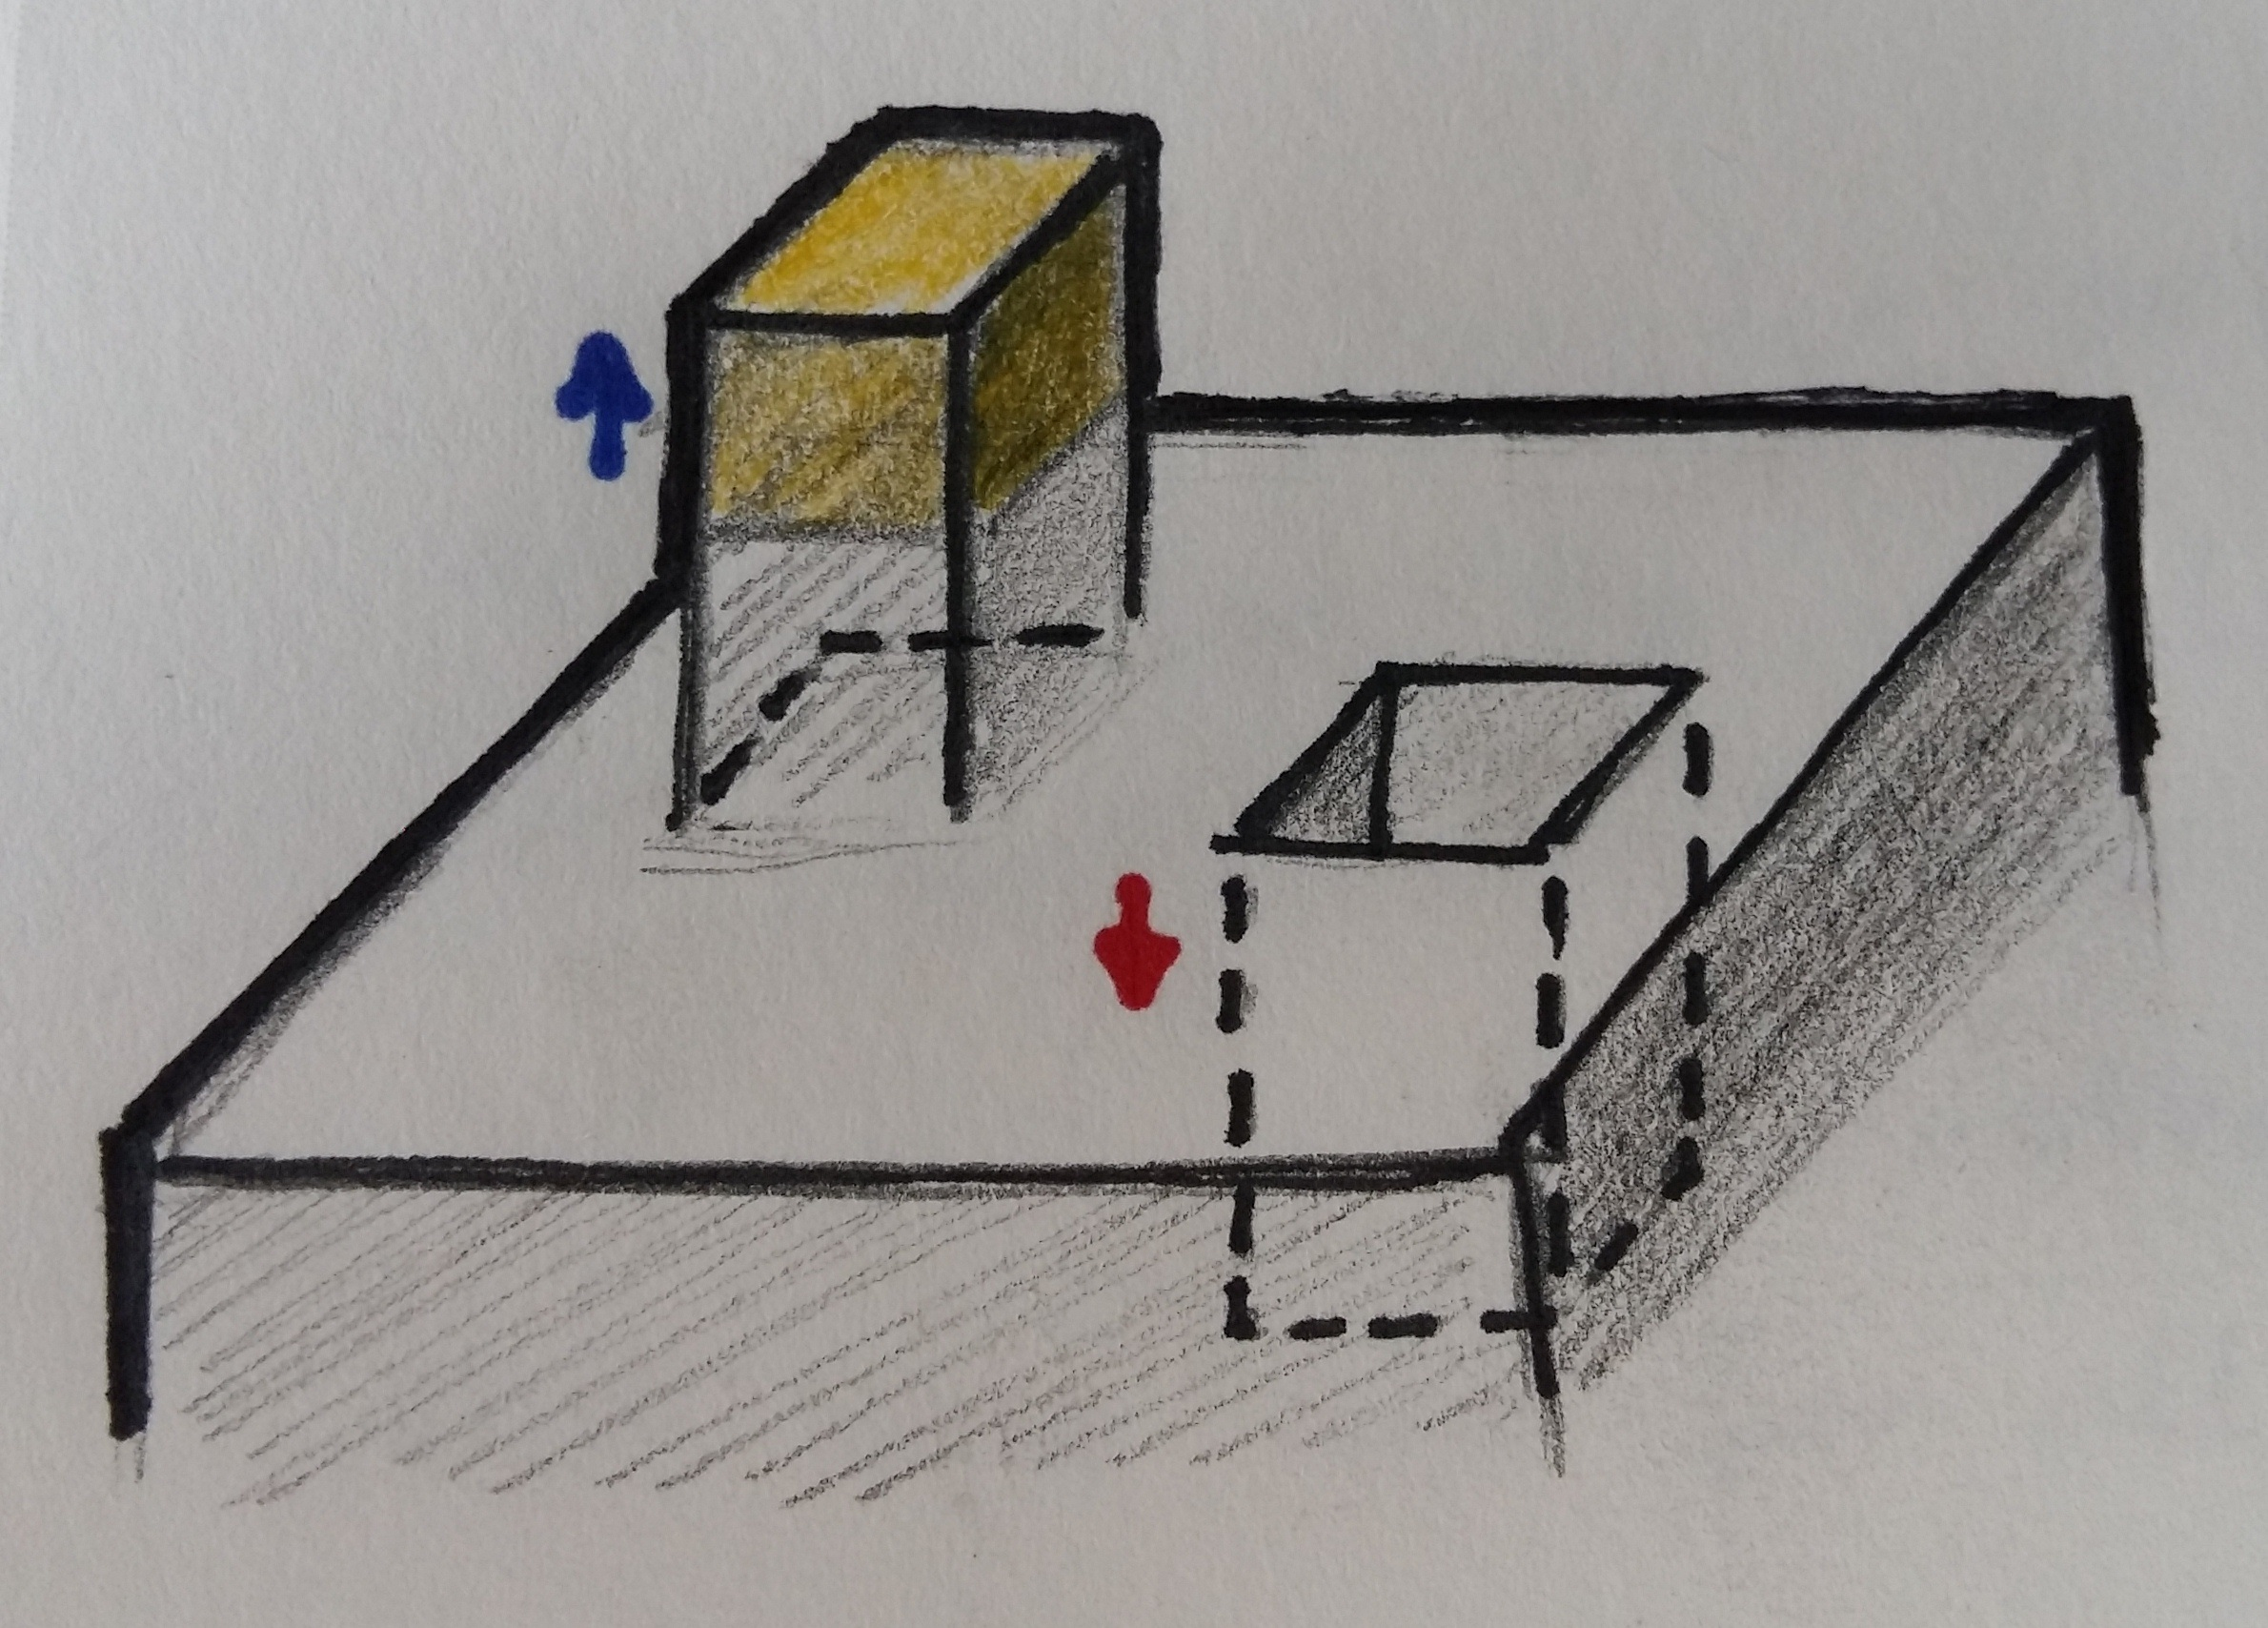
\includegraphics[width=0.5\textwidth]{draft1}
	\caption{conceitos iniciais}
\end{figure}


Foram então imaginados cenários que extrapolassem os usoss básicos das mecânicas propostas, de maneiras que se alinhassem aos conceitos pedagógicos que que deveriam ser transmitidos pelo jogo: desafios que dependessem da execução de tarefas em uma determinada ordem, em combinação com outras tarefas paralelas, ou dentro de um determinado limite de tempo. Nestes cenários, era esperado que jogadores conseguissem imaginar soluções mais sofisticadas, indo além das interações básicas às quais teriam acesso direto. Seria necessário movimentar massas de ar para jogar água contra blocos de terra, formando praias; escavar o solo para alcançar câmaras magmáticos e formar vulcões; ou alterar o curso de corpos d'água para formar cascatas.

\begin{figure}[h]
	\centering
	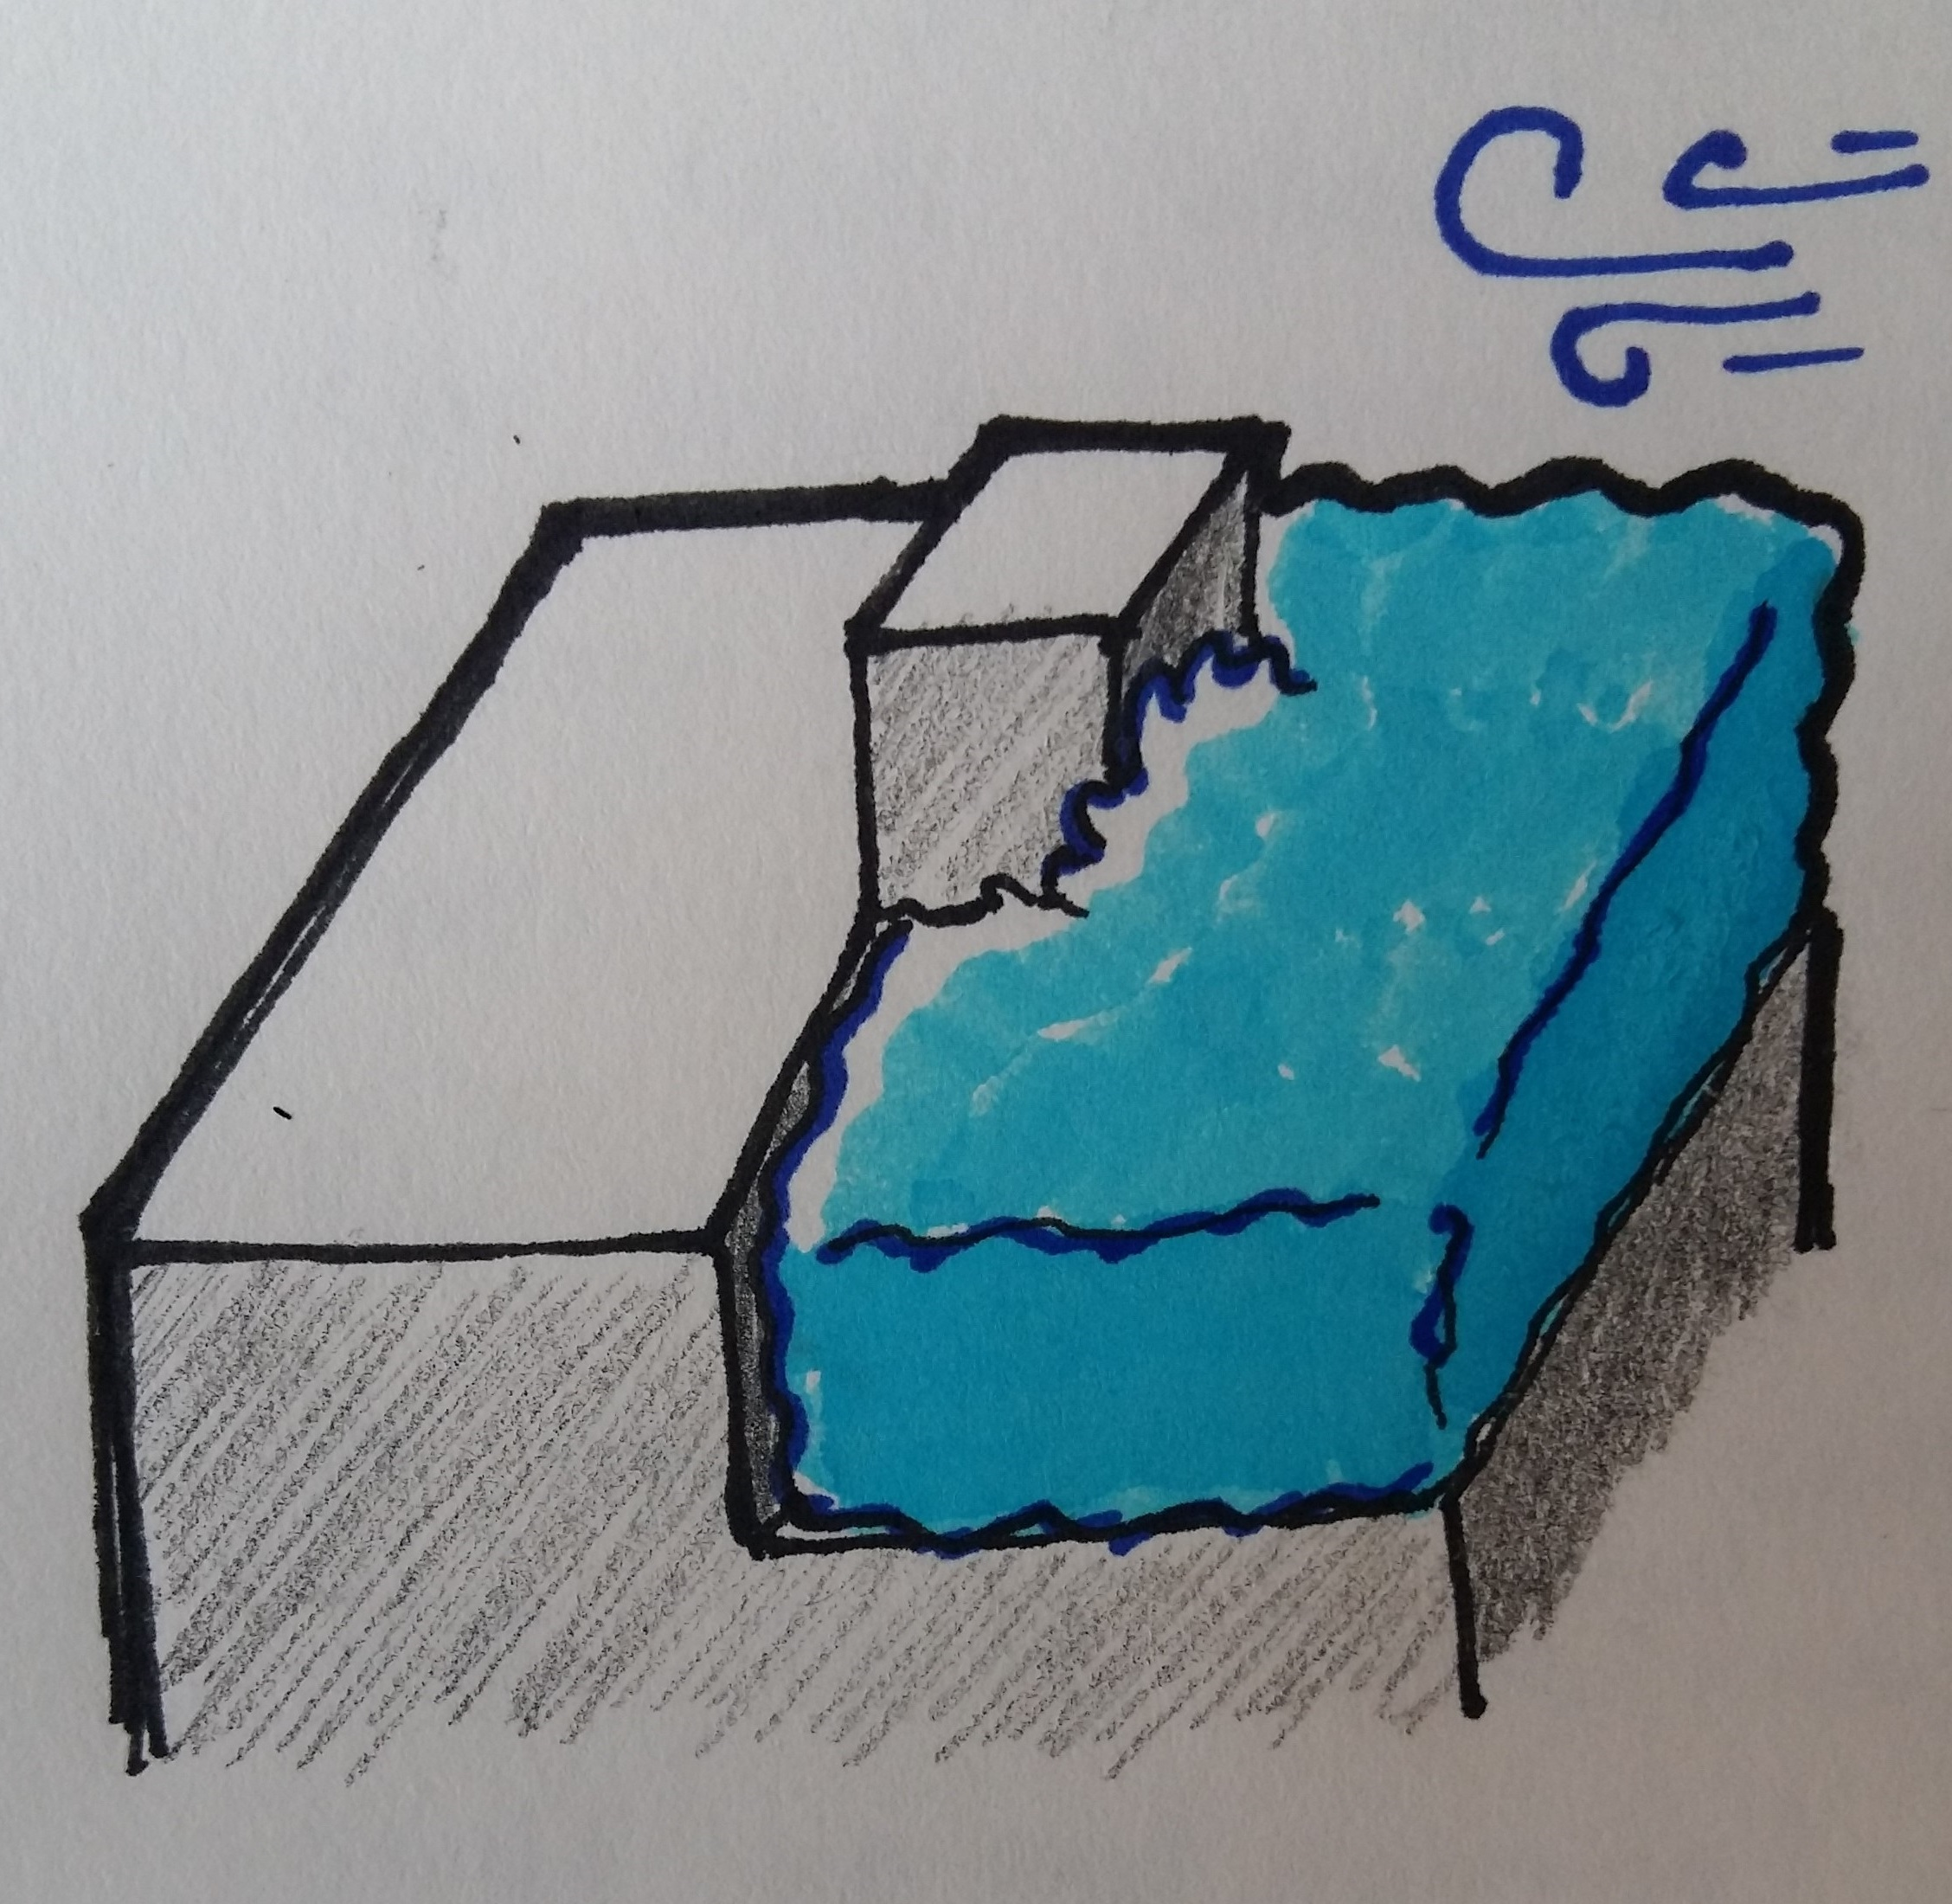
\includegraphics[width=0.5\textwidth]{draft2}
	\caption{primeiro rascunho do jogo}
\end{figure}

% ---
\section{Primeira iteração: prova de conceito}\label{sec-primeira-iteracao-prova-conceito}
% ---

Uma vez decidido o conceito a ser explorado, um pequeno protótipo foi proposto para dar ao grupo uma noção mais palpável de como esse jogo se pareceria, como seria controlá-lo, que dificuldades imprevistas apareceriam e quais as medidas que precisariam ser tomadas para suplantá-las. Este protótipo inicial tinha como objetivo tanto familiarizar o grupo às ferramentas e tecnologias escolhidas para a realização do trabalho quando ajudar a nivelar de maneira mais concreta a complexidade de sua implementação.

O protótipo deveria se ater apenas a uma mecânica básica da especificação do conceito: controle da elevação do terreno. O jogador teria acesso direto ao jogo - sem passar por telas de menu ou tutoriais - no qual se depararia com uma grade tridimensional de 5x5x5 cubos de terra, os quais poderia elevar ou rebaixar livremente.

\begin{figure}[h]
	\centering
	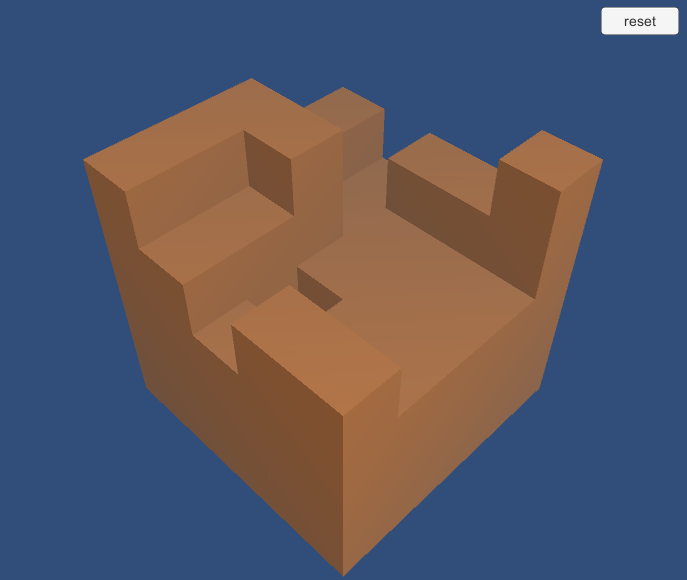
\includegraphics[width=0.5\textwidth]{ss1}
	\caption{prova de conceito do jogo}
\end{figure}

Apesar da simples implementação, algumas  primeiras dificuldades já puderam ser percebidas nesta iteração, sobretudo na integração dos dispositivos de realidade virtual.

A primeira barreira a ser percebida foi a falta de compatibilidade com dispositivos Android da versão mais recente do SDK do controlador Leap Motion, como havia nas versões anteriores. Isso, aliado ao fato de que a versão anterior do SDK não estava mais disponível para download, significou que uma interação direta entre o Leap Motion e o jogo compilado para dispositivos móveis não seria possível nessa etapa inicial do projeto.

Apesar deste empecilho, Unity se mostrou uma plataforma robusta e flexível o suficiente para a continuação do projeto, e as mecânicas básicas puderam ser implementadas rapidamente e sem grandes problemas.

% ---
\section{Segunda iteração: mecânicas básicas}\label{sec-segunda-iteracao-mecanicas-basicas}
% ---

Tendo em mente as facilidades e desafios percebidos durante a criação da prova de conceito, um segundo protótipo foi desenvolvido, desta vez com o intuito de acrescentar uma segunda mecânica básica - controle da precipitação - de modo a permitir que o jogador experimentasse com a interação entre as duas.

\begin{figure}[h]
	\centering
	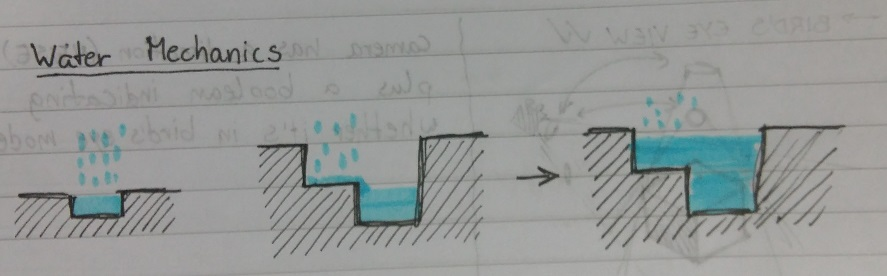
\includegraphics[width=0.5\textwidth]{water_mechanics1}
	\caption{mecânicas da água 1}
\end{figure}

\begin{figure}[h]
	\centering
	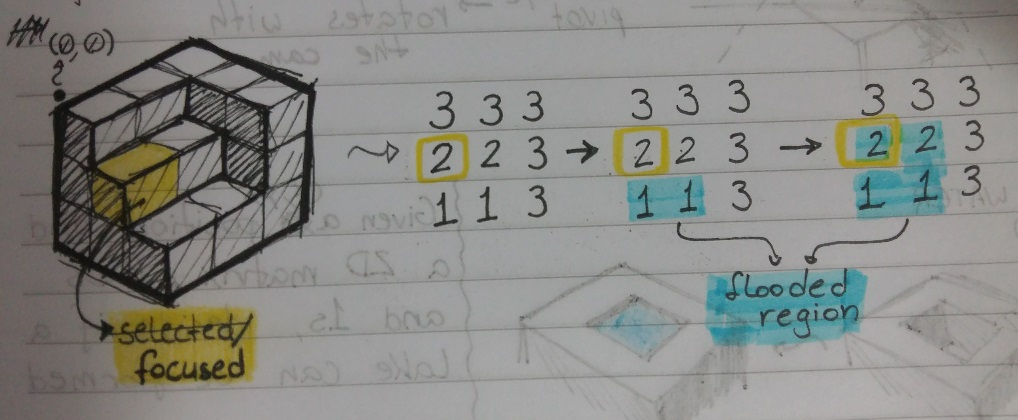
\includegraphics[width=0.5\textwidth]{water_mechanics2}
	\caption{mecânicas da água 2}
\end{figure}

Nesta iteração, haveria dois gestos que deveriam ser captados e interpretados pelo Leap Motion: abaixar e elevar a mão com a palma aberta para alterar a elevação do terreno e apontar todos os dedos para baixo para fazer chover em uma área específica.

\begin{figure}[h]
	\centering
	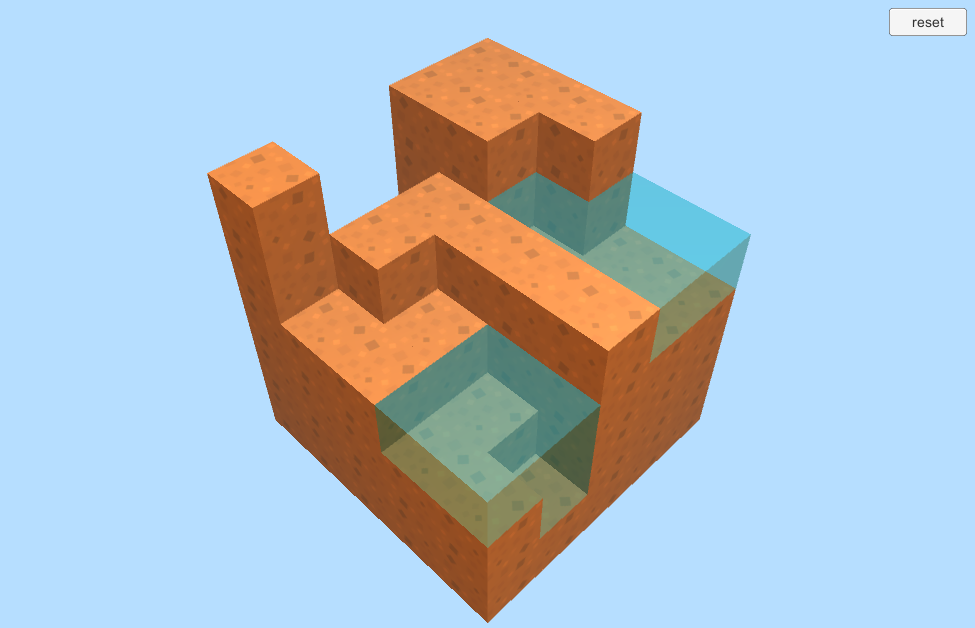
\includegraphics[width=0.5\textwidth]{ss2}
	\caption{prova de conceito do jogo}
\end{figure}

Durante a implementação dessas mecânicas, ficou clara a necessidade de uma mecânica de seleção que permitisse a manipulação de grandes áreas do terreno simultaneamente, então um terceiro gesto foi adicionado: pinçar e arrastar para delimitar áreas.

Também nessa etapa, percebeu-se que, devido à posição do Leap Motion, alguns dos gestos imaginados para as diferentes mecânicas do jogo - sobretudo o associado a chuva - não poderiam ser captados com a precisão necessária, nos levando a precisar reimaginar uma parte significativa da interação.


% ---
\section{Arquitetura}\label{sec-desenvolvimento-arquitetura}
% ---

Para se definir a arquitetura do sistema, é antes necessário identificar e entender cada um dos principais elementos, assim como suas interfaces.

% ---
\subsection{Identificação dos elementos}\label{subsec-identificacao-elementos}
% ---

% ---
\subsubsection{Controlador Leap Motion}\label{subsubsec-elemento-leapmotion}
% ---

Conforme visto em \ref{subsubsec-teo-leap-motion}, o controlador pode ser dividido em 2 elementos diferentes: O \textbf{hardware do controlador} e o \textbf{software} que aplica algoritmos de visão computacional nas imagens vindas do hardware, transformando-as em dados estruturados.

A parte de software pode ser executada no computador ou, no caso de se utilizar a versão 2 do SDK do Leap Motion, é possível utilizar a biblioteca beta para o Android.

% ---
\subsubsection{Lógica do jogo}\label{subsubsec-elemento-logica-jogo}
% ---

Este é o elemento que age sobre o ambiente virtual a partir de dados de entrada do controlador e do movimento do \textit{headset} de realidade virtual. Este elemento estará implementado no Unity, e pode ser executado ou no computador ou no próprio celular.

% ---
\subsubsection{Processamento de saída do video}\label{subsubsec-elemento-video}
% ---

Este elemento é controlado pelo SDK do Google Cardboard, e cuida de toda a parte de gerar a visão estereoscópica necessária para a visão 3D, além de movimentar a visão do jogo de acordo com o movimento do \textit{headset} de realidade virtual. Este elemento pode ser executado ou no computador ou no próprio celular.

% ---
\subsection{Arquiteturas estudadas}\label{subsec-arquiteturas-estudadas}
% ---

% ---
\subsubsection{Controlador diretamente conectado no celular}\label{subsubsec-arquiteturas-leapmotion-android}
% ---

A arquitetura que provê a maior mobilidade e que tem o menor número de subsistemas diferentes é aquele aonde se conecta o controlador Leap Motion diretamente ao celular, conforme mostrado na figura %TODO: Continue

\begin{figure}
	\centering
	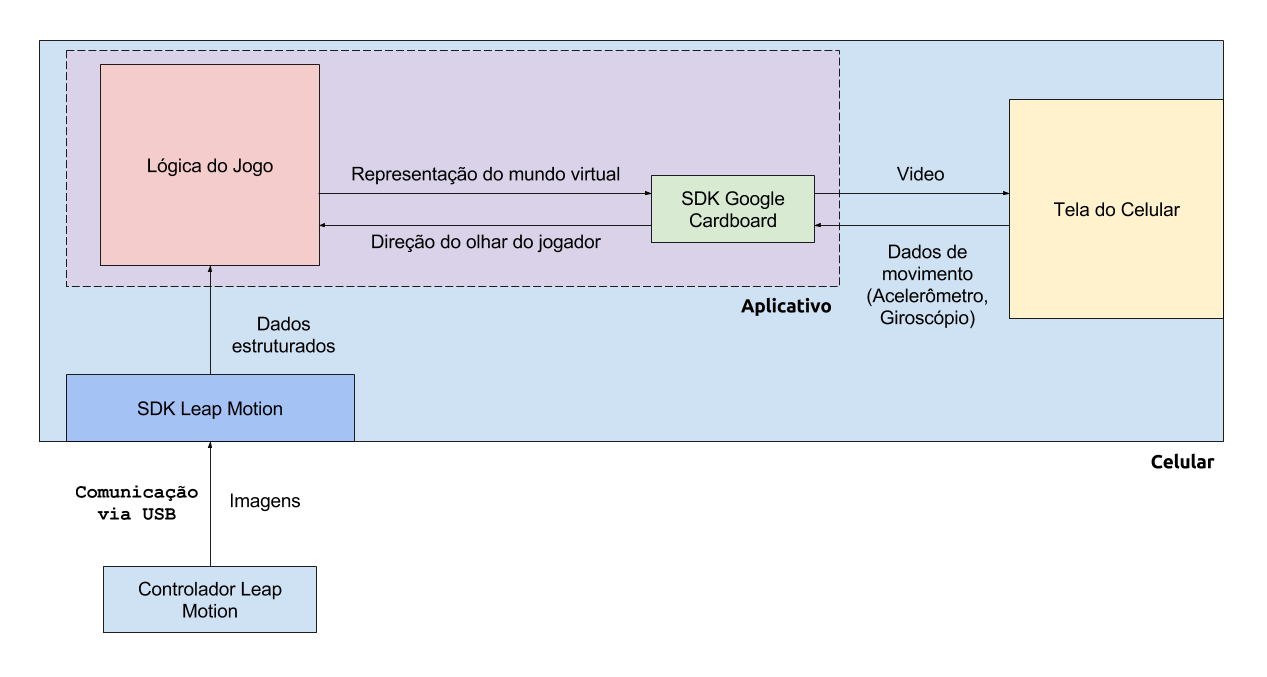
\includegraphics[width=0.7\linewidth]{images/Arquitetura-leap-android}
	\caption{}
	\label{fig:arquitetura-leap-android}
\end{figure}
